\chapter{R-Trees as a database level Nearest Neighbours Algorithm}

In MoodCat, the core function of the rooms is to find songs that fit to your mood. 
Finding these songs should be autonomous and accurate. 
In our development we opted to achieve this using a K-Nearest Neighbour (KNN) algorithm.

Such an algorithm finds the K nearest elements from a given point. 
Consider the room to be a point in 2D space (x axis is the valence vale, the y axis is the arousal value). 
For example, take the graphic below. 
The red dot is the room we're finding a song for, the green and blue dots are songs defined with a VA-Vector. 
The purple circle describes a KNN with K = 3, while the blue circle describes a KNN with K = 7. \\
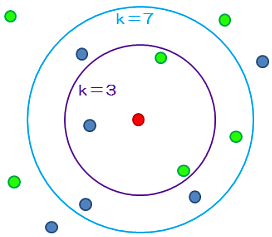
\includegraphics[scale=0.6]{knearestneighboursexample.png}\\

While developing MoodCat, we found that our initial, naive implementation slowed down drastically with a high amount of songs and rooms. 
We had to think of a different solution. 
Initially, we created an Approximate Nearest Neighbours (ANN) implementation using a KD-tree.
This remedies the slow runtime by calculating an approximate subset of points "sort of close" to the room.
On this subset our original NN algorithm could run.
Having solved the runtime complexity issues, we ran into memory issues instead.
Indexing all songs in a KD-tree still requires every song object to be loaded into memory.
We needed to find a sure-fire, effecient way of finding appropriate songs for a room.\\

We found the answer in the most unexpected part of the application: The database.
Specifically an R-tree index.
R-trees were proposed in 1984 by Antonin Guttman\footnote{http://www-db.deis.unibo.it/courses/SI-LS/papers/Gut84.pdf}. 
They provide reasonably fast and effecient storage and retrieval, and have the option to to a cheap K-NN like selection of the closest elements to a given point.
A good example of an application that uses this is OpenStreetMap\footnote{http://openstreetmap.org}.
They use PostGres spatial indexing (with r-trees) on all elements on their map.
With this, they decide what they should show at the current zoom level, as well as use it for route planning.

In MoodCat, we depend quite heavily on this concept.
Every room has a vector, and every song has a vector.
Both those vectors are indexed with r-trees.
To find fitting rooms to a given set of moods, we construct a vector from those moods and find the closest rooms in order of closeness.
In a room, we need to find fitting songs.
Again, we use r-trees to find songs with vectors closest to the room vector.

The reason r-trees are suitable for us to fix our scaling problems, is that the database does all the work.
This has the added benefit of the database being able to load only the tree to find the correct nodes, not the entire dataset.
This way we keep what we don't need on disk, and retrieve what we do need as fast as possible.